\chapter{Probability}
\label{probability}

\index{probability|(}

\section{Law of large numbers}

\subsection{Probability and the real world}
	Philosophically, probability can be connected to the real world via a principle from 1843:


	\begin{termBox}{\tBoxTitle{Cournot's principle}
	Very, very unlikely events simply do not happen.}
	\end{termBox}


	Some philosophers and others may disagree with this principle; we shall not try to settle the debate. But note that if we just say
	\begin{quote}
		Very, very unlikely events will happen very, very rarely...
	\end{quote}
	then it begs the question: what if they don't? What if 100 heads in a row occur when you toss a coin --- and the same happens to your friend? And your friend's friend? This should happen rarely indeed, but at what point do you put your foot down and declare it just should not happen? If we do not adopt Cournot's principle, probability theory is in danger of losing touch with reality.


	\index{random process|(}

	\begin{termBox}{\tBoxTitle{Probability}
	The \term{probability} of an outcome is the proportion of times the outcome would occur if we observed the random process an infinite number of times.}
	\end{termBox}

	Probability is defined as a proportion, and it always takes values between 0~and~1 (inclusively).
	It may also be displayed as a percentage between 0\% and 100\%.

	Probability can be illustrated by rolling a die many times.
	Let $\hat{p}_n$ be the proportion of outcomes $X_1,\dots,X_n$ that are \resp{1} after the first $n$ rolls:
	\[
		\hat p_n = \frac1n\sum_{i=1}^n X_i.
	\]
	As the number of rolls increases, $\hat{p}_n$ will converge to the probability of rolling a \resp{1}, $p = 1/6$.
	Figure~\ref{dieProp} shows this convergence for 100,000 die rolls.
	The tendency of $\hat{p}_n$ to stabilize around $p$ is described by the \term{Law of Large Numbers}. 

	\begin{figure}%[bt]
		\centering
		\includegraphics[width=0.85\textwidth]{ch_probability/figures/dieProp/dieProp}
		\caption{The fraction of die rolls that are 1 at each stage in a simulation.
		The proportion tends to get closer to the probability $1/6 \approx 0.167$ as the number of rolls increases.}
		\label{dieProp}
	\end{figure}

	\begin{termBox}{\tBoxTitle{Law of Large Numbers}
	As more observations are collected, the proportion $\hat{p}_n$ of occurrences with a particular outcome converges to the probability $p$ of that outcome.}
	\end{termBox}

	Occasionally the proportion will veer off from the probability and appear to defy the Law of Large Numbers, as $\hat{p}_n$ does many times in Figure~\ref{dieProp}. However, these deviations become smaller as the number of rolls increases.

	Above we write $p$ as the probability of rolling a \resp{1}. We can also write this probability as
	\begin{eqnarray*}
	\P(\text{rolling a \resp{1}})
	\end{eqnarray*}
	\marginpar[\raggedright\vspace{-13mm}

	$\P(A)$\vspace{1mm}\\\footnotesize Probability of\\outcome $A$]{\raggedright\vspace{-13mm}

	$\P(A)$\vspace{1mm}\\\footnotesize Probability of\\outcome $A$}As we become more comfortable with this notation, we will abbreviate it further. For instance, if it is clear that the process is ``rolling a die'', we could abbreviate $\P($rolling a \resp{1}$)$ as~$\P($\resp{1}$)$. 


	The Law of Large Numbers (LLN) comes in two flavors. The \term{strong LLN} says that for an infinite sequence of observations, with probability 1 the sequence $\hat p_n$ converges to $p$:
	\[
		\P(\lim_{n\to\infty}\hat p_n = p) = 1.
	\]
	The \term{weak LLN} says that as $n\to\infty$, the probability that $|\hat p_n-p|\ge\epsilon$ goes to 0, no matter how small $\epsilon$ is:
	\[
		\lim_{n\to\infty}\P(\hat p_n-p|<\epsilon) = 1.
	\]
	Both are true. The strong LLN is stronger (it says more, and it implies the weak LLN) but the strong LLN requires consideration of infinite sequences of outcomes, hence in applications it is sometimes conceptual ``overkill''.
	For students familiar with $\epsilon$-$\delta$ proofs, we offer:
	\begin{thm}
	The strong LLN implies the weak LLN.
	\end{thm}
	\begin{proof}
	Let $\epsilon>0$ be given. Since $\P(\lim_{n\to\infty}\hat p_n = p) = 1$,
	we have
	\[
		\P(\text{there is an $m$ such that for all $n\ge m$, $|\hat p_n-p|<\epsilon$})=1.
	\]
	Therefore for each $\delta>0$ there is an $m$ such that
	$\P(\text{for all $n\ge m$, $|\hat p_n-p|<\epsilon$})\ge 1-\delta$. In particular, for all $n\ge m$, $\P(|\hat p_n-p|<\epsilon)\ge 1-\delta$.
	\end{proof}

	\index{random process|)}

\subsection{Disjoint or mutually exclusive outcomes}
	\index{disjoint|(}
	\index{mutually exclusive|(}

	\term{Events} are \term{sets} of \term{outcomes}\footnote{The \emph{OpenIntro Statistics 3rd edition} text is not sufficiently clear on this important distinction, nor are many other statistics texts.}. You have perhaps encountered basic set theory in earlier mathematics courses.

	Two events $A$ and $B$ are called \term{disjoint} or \term{mutually exclusive} if they cannot both happen in the sense that they have no outcome in their intersection $A\cap B$ (``$A$ and $B$'').
	In this case we have $A\cap B=\emptyset$, the empty set. Thus, with $\cup$ or union meaning ``(inclusive) or'', the \term{Addition Rule} says
	\[
		\P(A\cup B) = \P(A) + \P(B) - \P(A\cap B),
	\]
	and if $A\cap B=\emptyset$ then $\P(A\cap B)=\P(\emptyset)=0$.

	We often abbreviate set notation in probability statements. Instead of
	\[
		\P(\{\omega: X(\omega)\le 3\})
	\]
	we may just write $\P(X\le 3)$ or even $\P(1\text{ or }2\text{ or }3)$ if the only possible outcomes that are at most 3 are 1, 2, and 3.
	Here the outcomes $\omega$ are drawn from the \term{sample space} $\Omega$ which is a set consisting of all possible outcomes.

	\begin{termBox}{\tBoxTitle{Addition Rule of disjoint outcomes} If $A_1$ and $A_2$ represent two disjoint outcomes, then the probability that one of them occurs is given by
	\begin{eqnarray*}
	\P(A_1\text{ or } A_2) = \P(A_1) + \P(A_2)
	\end{eqnarray*}
	If there are many disjoint outcomes $A_1,\dots,A_k$, then the probability that one of these outcomes will occur is
	\begin{eqnarray}
	\P(A_1) + \P(A_2) + \cdots + \P(A_k)
	\end{eqnarray}
	}
	\end{termBox}

	\index{event|(}

	Statisticians rarely work with individual outcomes and instead consider \indexthis{\emph{sets}}{sets} or \indexthis{\emph{collections}}{collections} of outcomes. Let $A$ represent the event where a die roll results in \resp{1} or \resp{2} and $B$~represent the event that the result is a \resp{4} or a \resp{6}. We write $A$ as the set of outcomes $\{$\resp{1},~\resp{2}$\}$ and $B=\{$\resp{4}, \resp{6}$\}$. These sets are commonly called \termsub{events}{event}. Because $A$ and $B$ have no elements in common, they are disjoint events. $A$ and $B$ are represented in Figure~\ref{disjointSets}.

	\begin{figure}%[hhh]
	\centering
	\includegraphics[width=0.55\textwidth]{ch_probability/figures/disjointSets/disjointSets}
	\caption{Three events, $A$, $B$, and $D$, consist of outcomes from rolling a die. $A$ and $B$ are disjoint since they do not have any outcomes in common. $B$ and $D$ are also disjoint.}
	\label{disjointSets}
	\end{figure}

	\begin{exercise}\label{lara}
	Can you modify $D$ in Figure \ref{disjointSets} to make $A$, $B$, $D$ pairwise disjoint?\footnote{Yes, let $D=\{3,5\}$, or more generally $D\subseteq\{3,5\}$.}
	\end{exercise}


	\index{event|)}
	\index{disjoint|)}
	\index{mutually exclusive|)}

	\begin{termBox}{\tBoxTitle{General Addition Rule} If $A$ and $B$ are any two events, disjoint or not, then the probability that at least one of them will occur is
	\begin{eqnarray}
	\P(A\text{ or }B) = \P(A) + \P(B) - \P(A\text{ and }B)
	\label{generalAdditionRule}
	\end{eqnarray}
	where $\P(A$ and $B)$ is the probability that both events occur.}
	\end{termBox}

	\begin{example}%Thanks to Christian
	Suppose we toss two coins. Let $A$ be the event that the 1st coin is heads, and $B$ the event that the 2nd coin is heads.
	Then the probability that at least one coin is heads is $\P(A\cup B)=\P(A)+\P(B)-\P(A\cap B)=\frac12+\frac12-\frac14 = \frac34$.
	\end{example}

\subsection{Probability distributions}



The \term{probability distribution} of a \term{random variable} $X:\Omega\to\mathbb R$ tells us what the probabilities of all events involving $X$ are: $\P(X\le 3)$, $\P(X=5)$, etc.

For continuous random variables, the probability of $X\in\mathcal A$ is calculated as
\[
	\P(X\in\mathcal A) = \int_{x\in \mathcal A} f(x)\,dx
\]
for a \term{probability density function} (pdf) $f$. In particular, the probability of any single particular outcome is zero. This may seem strange at first, but the idea can be seen as follows. If you measure somebody's height with infinite precision, the probability of anybody else having exactly the same height is zero.

The \term{cumulative distribution function} (cdf) $F$ is defined by
\[
	F(x)=\int_{-\infty}^x f(t)\,dt.
\]
\index{cdf|(}
\index{pdf|(}

\begin{termBox}{\tBoxTitle{Rules for probability distributions}
A probability distribution is a list of the possible outcomes with corresponding probabilities that satisfies three rules: \vspace{-2mm}
\begin{enumerate}
\setlength{\itemsep}{0mm}
\item The outcomes listed must be disjoint.
\item Each probability must be between 0 and 1.
\item The probabilities must total 1. \vspace{1mm}
\end{enumerate}}
\end{termBox}

\begin{figure}
\centering
\includegraphics[width=0.73\textwidth]{ch_probability/figures/diceSumDist/diceSumDist}
\caption{The probability distribution of the sum of two dice.}
\label{diceSumDist}
\end{figure}

In the bar plots Figure \ref{diceSumDist}, the bar heights represent the probabilities of outcomes. If the outcomes are numerical and discrete, it is usually (visually) convenient to make a bar plot that resembles a histogram, as in the case of the sum of two dice.

\subsection{Complement of an event}

Rolling a die produces a value in the set $\{$\resp{1}, \resp{2}, \resp{3}, \resp{4}, \resp{5}, \resp{6}$\}$. This set of all possible outcomes is called the \term{sample space} ($S$)\marginpar[\raggedright\vspace{-5mm}

$S$\\\footnotesize Sample space]{\raggedright\vspace{-5mm}

$S$\\\footnotesize Sample space}\index{S@$S$} for rolling a die. We often use the sample space to examine the scenario where an event does not occur.

Let $D=\{$\resp{2}, \resp{3}$\}$ represent the event that the outcome of a die roll is \resp{2} or \resp{3}. Then the \term{complement}\marginpar[\raggedright\vspace{0.2mm}

$A^c$\\\footnotesize Complement\\of outcome $A$]{\raggedright\vspace{0.2mm}

$A^c$\\\footnotesize Complement\\of outcome $A$}\index{Ac@$A^c$} of $D$ represents all outcomes in our sample space that are not in $D$, which is denoted by $D^c = \{$\resp{1}, \resp{4}, \resp{5}, \resp{6}$\}$. That is, $D^c$ is the set of all possible outcomes not already included in $D$.

%Figure~\ref{complementOfD} shows the relationship between $D$, $D^c$, and the sample space $S$. 
%\begin{figure}[hht]
%\centering
%\includegraphics[width=0.55\textwidth]{ch_probability/figures/complementOfD/complementOfD}
%\caption{Event $D=\{$\resp{2}, \resp{3}$\}$ and its complement, $D^c = \{$\resp{1}, \resp{4}, \resp{5}, \resp{6}$\}$. $S$~represents the sample space, which is the set of all possible outcomes.}
%\label{complementOfD}
%\end{figure}


A complement of an event $A$ is constructed to have two very important properties: (i) every possible outcome not in $A$ is in $A^c$, and (ii) $A$ and $A^c$ are disjoint. Property (i) implies
\begin{eqnarray}
\P(A\text{ or }A^c) = 1
\label{complementSumTo1}
\end{eqnarray}
That is, if the outcome is not in $A$, it must be represented in $A^c$. We use the Addition Rule for disjoint events to apply Property (ii):
\begin{eqnarray}
\P(A\text{ or }A^c) = \P(A) + \P(A^c)
\label{complementDisjointEquation}
\end{eqnarray}
Combining Equations~(\ref{complementSumTo1}) and~(\ref{complementDisjointEquation}) yields a very useful relationship between the probability of an event and its complement.

\begin{termBox}{\tBoxTitle{Complement}
The complement of event $A$ is denoted $A^c$, and $A^c$ represents all outcomes not in~$A$. $A$ and $A^c$ are mathematically related: \vspace{-2mm}
\begin{eqnarray}\label{complement}
\P(A) + \P(A^c) = 1, \quad\text{i.e.}\quad \P(A) = 1-\P(A^c)
\end{eqnarray}\vspace{-6.5mm}}
\end{termBox}

In simple examples, computing $A$ or $A^c$ is feasible in a few steps. However, using the complement can save a lot of time as problems grow in complexity.


\section{Independence and conditional probability}
\label{probabilityIndependence}

\index{conditional probability|(}
\label{conditionalProbabilitySection}
\paragraph{Conditional probability.}
Suppose we don't know the outcome of our probability experiment, we only know that the event $B\subseteq\Omega$ occurred.
Then it makes sense to replace $\Omega$ by $B$, since the sample space should consist of all ``possible'' outcomes, and only the outcomes in $B$ are still possible.
The probabilities in this space should be given by
\[
	\P(A\text{ given }B) = \P(A\mid B) = \frac{\P(A\cap B)}{\P(B)}
\]
since this represents the fraction of the ``probability mass'' in $B$ that is in $A$. To put it another way, if we run the probability experiment associated with $\Omega$ many times, this is the long-term fraction of times $A\cap B$ occurs, divided by the long-term fraction of time $B$ occurs. In other words, it is the long-term fraction of times that $A$ occurs, \emph{out of} the times that $B$ occurs\footnote{Here ``long-term'' should be understood in the context of Cournot's Principle and the Law of Large Numbers.}

Once we have this, independence of $A$ and $B$ is given by
\[
	\P(A\mid B) = \P(A),
\]
i.e., the knowledge that $B$ occurs does not affect our probability that $A$ occurs.
\begin{exercise}
	Under what conditions is this equivalent to
	\[
		\P(B\mid A) = \P(B)?\footnote{If $\P(B)=0$ or $\P(A)=0$ then they cannot be equivalent, as they will not both be defined. However, once both probabilities are nonzero, both equations are just expressing that $\P(A\cap B)=\P(A)\P(B)$.}
	\]
\end{exercise}

\begin{termBox}{\tBoxTitle{\term{Multiplication Rule} for independent processes}
If $A$ and $B$ represent events from two different and independent processes, then the probability that both $A$ and $B$ occur can be calculated as the product of their separate probabilities: \vspace{-1.5mm}
\begin{eqnarray}\label{eqForIndependentEvents}
\P(A \text{ and }B) = \P(A) \times  \P(B)
\end{eqnarray}
Here and elsewhere in \emph{OpenIntro Statistics} and in the present text, $\times$ is used to denote multiplication.

Similarly, if there are $k$ events $A_1,\dots,A_k$ from $k$ independent processes, then the probability they all occur is\vspace{-1.5mm}
\begin{eqnarray*}
\P(A_1) \times  \P(A_2)\times  \cdots \times  \P(A_k)
\end{eqnarray*}\vspace{-6mm}}
\end{termBox}


Sometimes we wonder if one outcome provides useful information about another outcome. The question we are asking is, are the occurrences of the two events independent? We say that two events $A$ and $B$ are independent if they satisfy Equation~\eqref{eqForIndependentEvents}.


%_________________

\subsection{Marginal and joint probabilities}
\label{marginalAndJointProbabilities}

\index{marginal probability|(}
\index{joint probability|(}

When random variables $X$ and $Y$ are \term{jointly distributed}, i.e., they are defined on the same sample space $\Omega$ with the same probabilities for events in $\Omega$, we can speak of probabilities involving them both, such as
\[
	\P(X<Y)
\]
This is an example of joint probability.
For non-continuous (discrete) random variables, we can then discuss $M(x)=\P(X=x)$ for particular values of $x$. This is the \term{probability mass function} of $X$. When also discussing $Y$ and possibly other random variables that are jointly distributed with $X$, it is also called the \term{marginal distribution} of $X$. The function $M(x,y)=\P(X=x\text{ and } Y=y)$ is then the \term{joint probability mass function} of $X$ and $Y$. Since $Y$ must take \emph{some} value, we can compute
\[
	\P(X=x) = \sum_y \P(X=x \text{ and }Y=y).
\]
If we make a table with $x$ and $y$ axes this hints at why the term ``marginal'' is used: each axis is a margin.

%\begin{termBox}{\tBoxTitle{Marginal and joint probabilities}
%If a probability is based on a single variable, it is a \emph{\hiddenterm{marginal probability}}. The probability of outcomes for two or more variables or processes is called a \emph{\hiddenterm{joint probability}}.}
%\end{termBox}




\begin{table}%[h]
\centering
\begin{tabular}{ll rr r}
& & \multicolumn{2}{c}{$X$} & \\
\cline{3-4}
& & $X=1$ &$X=0$ & Total  \\
   \cline{2-5}
 & $Y=1$     & 0.0382 & 0.8252 & 0.8634 \\
\raisebox{1.5ex}[0pt]{\var{$Y$}} & $Y=0$ \hspace{0.5cm} & 0.0010 & 0.1356  & 0.1366  \\
   \cline{2-5}
& Total & 0.0392 & 0.9608 & 1.0000 \\
\end{tabular}
\caption{Joint probability table. Compare to the \data{smallpox} table in the main text.\textC{\vspace{-2mm}}}
\label{smallpoxProbabilityTable}
\end{table}


%\subsection{General multiplication rule}
%Section~\ref{probabilityIndependence} introduced the Multiplication Rule for independent processes.
%Here we provide the \term{General Multiplication Rule} for events that might not be independent.

%\begin{termBox}{\tBoxTitle{General Multiplication Rule}
%If $A$ and $B$ represent two outcomes or events, then \vspace{-1.5mm}
%\begin{eqnarray*}
%P(A\text{ and }B) = P(A | B)\times P(B)
%\end{eqnarray*} \vspace{-6.5mm} \par
%It is useful to think of $A$ as the outcome of interest and $B$ as the condition.}
%\end{termBox}
%This General Multiplication Rule is simply a rearrangement of the definition for conditional probability in Equation~(\ref{condProbEq}) on page~\pageref{condProbEq}.


\begin{termBox}{\tBoxTitle{Sum of conditional probabilities}
Let $A_1,\dots,A_k$ represent all the disjoint outcomes for a variable or process. Then if $B$ is an event, possibly for another variable or process, we have: \vspace{-1mm}
\begin{eqnarray*}
\P(A_1|B)+\cdots+\P(A_k|B) = 1
\end{eqnarray*}\vspace{-5.5mm} \par
The rule for complements also holds when an event and its complement are conditioned on the same information: \vspace{-1.5mm}
\begin{eqnarray*}
\P(A | B) = 1 - \P(A^c | B)
\end{eqnarray*}}
\end{termBox}

\subsection{Independence considerations in conditional probability}

If two events are independent, then knowing the outcome of one should provide no information about (\emph{the probability of!}) the other. We can show this is mathematically true using conditional probabilities.

\begin{exercise}
	Can you think of a situation where we have events $A$, $B$, $C$ such that $A$ and $B$ are independent, but nevertheless neither one is independent of $C$?\footnote{Let $A$ and $B$ be the events that two spouses win on their lottery tickets (assume they are playing different lotteries, so that $A$ and $B$ can be independent). Then $A$ and $B$ both influence the event $C$ that the family becomes richer than before.}
\end{exercise}

%\subsection{Tree diagrams}
%\index{data!smallpox|)}
\index{tree diagram|(}

\termsub{Tree diagrams}{tree diagram} are a tool to organize outcomes and probabilities around the structure of the data.  Figure~\ref{smallpoxTreeDiagram} shows the general idea.
\begin{figure}%[ht]
\centering
\includegraphics[width=0.93\textwidth]{ch_probability/figures/smallpoxTreeDiagram/smallpoxTreeDiagram}
\caption{A tree diagram of the \data{smallpox} data set. To make this abstract, consider $\P(X=1)=0.0392$ to be ``inoculated? yes, 0.0392'', $X=0$ to be ``no, not inoculated'', $\P(Y=1\mid X=1)=0.9754$ is then ``lived, 0.9754'' and so on.}
\label{smallpoxTreeDiagram}
\end{figure}



\subsection{Bayes' Theorem}
\label{bayesTheoremSubsection}

\index{Bayes' Theorem|(}

It is a consequence of the definition of conditional probability and the fact that $\P(A) = \P(A\cap B) + \P(A\cap B^c)$. And that more generally, if $B_i$ are disjoint with $\bigcup_i B_i=\Omega$, then
\[
	\P(A) = \sum_i \P(A\cap B_i).
\]
Even though that may sound easy enough, it takes some practice to successfully solve Bayes Theorem problems in a reasonable amount of time.

\begin{termBox}{\tBoxTitle{Bayes' Theorem: inverting probabilities}
Consider the following conditional probability for variable 1 and variable 2:\vspace{-1.5mm}
\begin{align*}
\P(\text{outcome $A_1$ of variable 1 } | \text{ outcome $B$ of variable 2})
\end{align*}
Bayes' Theorem states that this conditional probability can be identified as the following fraction:\vspace{-1.5mm}
\begin{align}
\frac{\P(B | A_1) \P(A_1)}
	{\P(B | A_1) \P(A_1) + \P(B | A_2) \P(A_2) + \cdots + \P(B | A_k) \P(A_k)}
	\label{equationOfBayesTheorem}
\end{align}
where $A_2, A_3, \dots, A_k$ represent all other possible outcomes of the first variable.}\index{Bayes' Theorem|textbf}
\end{termBox}

Bayes' Theorem is just a generalization of what we have done using tree diagrams. The numerator identifies the probability of getting both $A_1$ and $B$. The denominator is the marginal probability of getting $B$. This bottom component of the fraction appears long and complicated since we have to add up probabilities from all of the different ways to get $B$. We always completed this step when using tree diagrams. However, we usually did it in a separate step so it didn't seem as complex.

To apply Bayes' Theorem correctly, there are two preparatory steps:
\begin{enumerate}
\setlength{\itemsep}{0mm}
\item[(1)] First identify the marginal probabilities of each possible outcome of the first variable: $\P(A_1), \P(A_2),\dots \P(A_k)$.
\item[(2)] Then identify the probability of the outcome $B$, conditioned on each possible scenario for the first variable: $\P(B | A_1), \P(B | A_2), \dots, \P(B | A_k)$.
\end{enumerate}
Once each of these probabilities are identified, they can be applied directly within the formula.

%\begin{tipBox}{\tipBoxTitle{Only use Bayes' Theorem when tree diagrams are difficult}
%Drawing a tree diagram makes it easier to understand how two variables are connected. Use Bayes' Theorem only when there are so many scenarios that drawing a tree diagram would be complex.}
%\end{tipBox}



\index{Bayes' Theorem|)}
\index{tree diagram|)}
\index{conditional probability|)}
\index{probability|)}

\subsection{Sampling from a small population}
\label{smallPop}

It is time to remind you of the notation
\[
	\bar w = www\dots
\]
used in repeated decimal expansions.
In particular, you should find it useful to know the expansions in Table \ref{142857}.
\begin{table}
\centering
\begin{tabular}{| l | l | l | l | l | l |} %weird mixture of L's and bars
\hline
	$1/1=1$	& $1/2=.5$ 			&  $1/3=.\bar 3$	&  $1/4=.25$	& $1/5=.2$ 	& $1/6=.1\bar 6$ \\
	$1/7=.\overline{142857}$ 	& $1/8=.125$		& $1/9=.\bar 1$	& $1/10 = .1$	& $1/11=.\overline{09}$	& $1/12=.08\bar 3$.\\
\hline
\end{tabular}
\caption{Few people know by heart what $1/13$ is, but $1/n$ for smaller $n$ are listed here.}\label{142857}
\end{table}


We now discuss \term{sampling without replacement} and \term{with replacement}.

Suppose we pick two marbles out of a jar of $n$ marbles, without replacement. Suppose $b$ many of the marbles in the jar are blue.
The probability that the two marbles we picked are both blue is
\[
	\frac{b}{n}\cdot \frac{b-1}{n-1}.\tag{1}
\]
If we replaced the first one before picking the second time,
\[
	\frac{b}{n}\cdot \frac{b}{n}.\tag{2}
\]
\begin{exercise}
True or false: If the population is large, so that $n$ and $b$ are both large, then the difference between (1) and (2) is negligible.\footnote{
True. Since $b\le n$, we have
\[
	\left | \frac{b-1}{n-1}  - \frac{b}{n} \right| = \frac{|n(b-1)-(n-1)b|}{n(n-1)} = \frac{n-b}{n(n-1)} \le \frac{1}{n-1}
\]
which goes to zero as $n\to\infty$.
}
\end{exercise}


\section{Bayesian statistics}

Suppose we have a Bernoulli distribution with parameter $p$, which is unknown.
Perhaps we should take $p=1/2$ as our starting assumption (this is consistent with the idea of maximum entropy from Section \ref{maxEnt}).
Now suppose we observe $X=1$ (heads). Then we can \emph{update} our estimate of $p$ as follows, in the spirit of Bayes' Theorem:
\[
	\P(p=p_0\mid X=1) = \frac{\P(X=1\mid p=p_0)\cdot \P(p=p_0)}{\P(X=1)}
\]
However, if we consider $p$ to be a random variable, then any particular value will have probability 0 and we should be considering the \term{probability density function} (see Section~\ref{contDist}) instead:
\begin{equation}\label{learnBayes}
	f_p(p_0\mid X=1) = \frac{\P(X=1\mid p=p_0)\cdot f_p(p_0)}{\P(X=1)}.
\end{equation}
So let us not assume $p=1/2$ to start, but instead take $f_p(x)=1$ for each $0\le x\le 1$, which we write as
\[
f_p(x)=1_{[0,1]}(x).
\]
This reflects us having no prior knowledge of what $p$ might be.
Now $\P(X=1\mid p=p_0)$ is supposed to be $p_0$ (even though $p=p_0$ is a probability-zero event, which leads to dividing by zero if we literally using it in conditional probability)
because, if $\P(X=1)=p=p_0$ if $p=p_0$. So we get
\[
	f_p(p_0\mid X=1) = p_0 \cdot 1_{[0,1]}(p_0)/(1/2) = 2p_0\cdot 1_{[0,1]}(p_0).
\]
If we now make another observation, we can repeat this process starting with our new pdf and get yet another one.
Namely, let's say $f_0(x)=1_{[0,1]}(x)$ and $f_1(x)=2x\cdot 1_{[0,1]}(x)$.
Then if our next observation is $X=0$, we get
\begin{eqnarray*}
	f_2(p_0) &=& f_1(p_0\mid X=0)\\
	&=& \P(X=0\mid p=p_0)f_p(p_0)/\P(X=0) = (1-p_0) 2p_0 / (1/3) = 6p_0(1-p_0).
\end{eqnarray*}
Here we have used
\begin{eqnarray*}
	\P(X=0)&=&\int \P(X=0\mid p_0)f_1(p_0)\,dp\\
	&=& \int (1-p_0)2p_0\, dp = 2(1/2-1/3) = 1/3.
\end{eqnarray*}


We see that $f_2$ has its mode at $p_0=1/2$, which is reasonable since we have observed one heads and one tails.
On the other hand, the variance of $f_2$ is smaller than that of $f_0$, which is also reasonable since we have more observations to go by:
\begin{eqnarray*}
	\Var(p) = \E(p^2)-\E(p)^2 &=& \int_0^1 p^2 (6p(1-p))\,dp - (1/2)^2\\
	& =& 6\left(\frac14-\frac15\right)-\frac14 = \frac6{20}-\frac14 = \frac1{20} < \frac13-\frac14 = \frac1{12}.
\end{eqnarray*}

We will not go deeply into Bayesian statistics in this book, but suffice it to say that philosophically, there are at least two possible approaches to probability and statistics:
\begin{itemize}
\item \term{Frequentist statistics} holds that probabilities like $p$ above are estimated from a sample $\hat p=\sum X_i/n$;
\item \term{Bayesian statistics} holds that rather than an infinitely precise estimate value $\hat p$, we have a pdf representing our current beliefs about what $p$ might be. This pdf becomes more sharply peaked as we gather more sample points.
\end{itemize}
While the frequentist stance avoids the tricky issue ``what should our initial pdf, after seeing 0 values, be?'', the Bayesian stance is well-suited to machine learning, whereby a machine can be continuously updating its beliefs about the world using the method of (\ref{learnBayes}).

%_________________
%_________________
\section{Random variables}
\label{randomVariablesSection}

\index{random variable|(}


\subsection{Expectation}

\index{expectation|(}

Just like probability is a long-term proportion, expectation is a long-term average.

We call a variable or process with a numerical outcome a \term{random variable}, and we usually represent this random variable with a capital letter such as $X$, $Y$, or $Z$.
Actually a random variable could take values that are vectors, functions and several other things. The main requirement is that we have a function $X:\Omega\to \mathcal A$ where $\Omega$ is our sample space, and probability enters the picture as $\P(X\in A)=\P(\{\omega\in\Omega:X(\omega)\in\mathcal A\})$.

%\begin{termBox}{\tBoxTitle{Random variable}
%A random process or variable with a numerical outcome.}
%\end{termBox}


We compute the average outcome of $X$ and call this average the \term{expected value} of $X$, denoted by $\E(X)$\index{EX@$\E(X)$}\marginpar[\raggedright\vspace{-3mm}

$\E(X)$\vspace{1mm}\\\footnotesize Expected\\value of $X$]{\raggedright\vspace{-3mm}

$\E(X)$\vspace{1mm}\\\footnotesize Expected\\value of $X$}. The expected value of a random variable is computed by adding each outcome weighted by its probability, for instance:
\begin{align*}
\E(X) &= 0 \times  \P(X=0) + 137 \times  \P(X=137) + 170 \times  \P(X=170) \\
	&= 0 \times  0.20 + 137 \times  0.55 + 170 \times  0.25 = 117.85
\end{align*}

\begin{termBox}{\tBoxTitle{Expected value of a Discrete Random Variable}
If $X$ takes outcomes $x_1,\dots, x_k$ with probabilities $\P(X=x_1),\dots, \P(X=x_k)$, the expected value of $X$ is the sum of each outcome multiplied by its corresponding probability:
\begin{align}
\E(X) 	&= x_1\times \P(X=x_1) + \cdots + x_k\times \P(X=x_k) \notag \\
	&= \sum_{i=1}^{k}x_i\P(X=x_i)
\end{align}
The Greek letter $\mu$\index{Greek!mu ($\mu$)} may be used in place of the notation $\E(X)$.}
\end{termBox}

It is also possible to compute the expected value of a continuous random variable (see Section~\ref{contDist}):
\[
\mu = \int xf(x)dx
\]
where $f(x)$, the probability density function, represents a function for the density curve.


\begin{figure}
\centering
\includegraphics[width=0.68\textwidth]{ch_probability/figures/contBalance/contBalance}
\caption{A continuous distribution balanced at its mean.}
\label{contBalance}
\end{figure}

\index{expectation|)}


The \term{(sample) mean}, sometimes called the (sample) \indexthis{average}{mean!average} of a data set $x_1,\dots,x_n$ is distinct from the mean of a random variable.

However, we can ``freeze'' a data set and consider the uniform distribution on it.
\begin{df}
The \term{uniform distribution} on a finite set of $n$ elements, $\{x_1,\dots,x_n\}$, is given by $\P(X=x_i)=\frac1n$. If some of the $x_i$ are identical (say $k$ many are equal to a particular $x_i$) this makes that element have probability $k/n$.
\end{df}
\begin{example}{The uniform distribution on $\{1.3, 2.0, -4\}$.}
This distribution is such that if a variable $X$ has this distribution then $\P(X=1.3)=1/3$, $\P(X=2.0)=1/3$, and $\P(X=-4)=1/3$.
\end{example}

In this case the sample mean of the original data set becomes the mean of the new random variable. The sample standard deviation of the original data set does not quite become the standard deviation of the new random variable. Indeed, if we have just a single data point, the sample standard deviation is (rightly so) undefined, as it tells us nothing about the underlying standard deviation; but the frozen distribution has standard deviation 0.

In the sample standard deviation from Chapter 1, we divide by $n-1$, rather than dividing by $n$. This way, the expectation of the sample variance turns out to be the original distribution's variance. Indeed, define the random variable $S$ by
\[
	S^2 = \frac1n \sum_{i=1}^n (X_i-\bar X)^2.
\]
\begin{thm}
$\E(S^2)=\sigma^2$.
\end{thm}
\begin{proof}
Let us make the simplifying assumption that $\E(X_i)=0$.
The value of
\[
	\E\left (\sum_{i=1}^n (X_i-\bar X)^2\right)
\]
is obtained by
\begin{eqnarray*}
	\E((X_i-\bar X)^2) &=& \E(X_i^2-2X_i\bar X + (\bar X)^2)\\
	&=& \underbrace{\E(X_i^2)}_{\text{first term}}-2\underbrace{\E(X_i\bar X)}_{\text{second term}} + \underbrace{\E((\bar X)^2)}_{\text{third term}}
\end{eqnarray*}
The first term is $\sigma^2$.
The second term is
\[
\E(X_i\bar X) = \frac1n \sum_j \E(X_iX_j) = \frac1n \E(X_iX_i) = \frac1n \sigma^2.
\]
The third term is found using
\[
	\E(n^2(\bar X)^2) = \E\left (\left (\sum_{i=1}^n X_i\right )^2\right) = \E\left (\sum_i X_i^2 + \sum_{i\ne j} X_iX_j\right)
	%= \E\left (\sum_i X_i^2 + 2\sum_{i<j} X_iX_j\right )
\]
\[
	= \E\left (\sum_i X_i^2 + 2\sum_{i<j} X_iX_j\right ) = n(\sigma^2)
\]
to be $\E((\bar X)^2) = \sigma^2/n$. Thus
\begin{eqnarray*}
	\E((X_i-\bar X)^2) %= \E(X_i^2-2X_i\bar X + (\bar X)^2) = \sigma^2-2\E(X_i\bar X) + \sigma^2/n\\
	= \sigma^2-2\sigma^2/n + \sigma^2/n = \sigma^2\left(1-\frac1n\right) = \sigma^2\cdot\frac{n-1}n.
\end{eqnarray*}
Consequently,
%\[
%	\E\left (\frac1n\sum_i (X_i-\bar X)^2\right) = \E\left((X_1-\bar X)^2\right) = \sigma^2\cdot\frac{n-1}n,
%\]
%and so of course
\[
\E\left(\frac1{n-1}\sum_i (X_i-\bar X)^2\right) = \sigma^2.\qedhere
\]
\end{proof}

\subsection{Variability in random variables}

\begin{termBox}{\tBoxTitle{General variance formula}
If $X$ takes outcomes $x_1,\dots x_k$ with probabilities $\P(X=x_1),\dots, \P(X=x_k)$ and expected value $\mu=\E(X)$, then the variance of $X$, denoted by $\Var(X)$ or the symbol $\sigma^2$, is
\[
\sigma^2 = \sum_{j=1}^{k} (x_j - \mu)^2 \P(X=x_j)
\]
The standard deviation of $X$, labeled $\sigma$\index{Greek!sigma ($\sigma$)} or $\SD(X)$, is the square root of the variance.}
\end{termBox}
\marginpar[\raggedright\vspace{-47mm}

$\Var(X)$\vspace{1mm}\\\footnotesize Variance\\of $X$]{\raggedright\vspace{-47mm}

$\Var(X)$\vspace{1mm}\\\footnotesize Variance\\of $X$}


\subsection{Linear combinations of random variables}

	Two important concepts concerning combinations of random variables have so far been introduced. First, a final value can sometimes be described as the sum of its parts in an equation. Second, intuition suggests that putting the individual average values into this equation gives the average value we would expect in total. This second point needs clarification -- it is guaranteed to be true in what are called \emph{linear combinations of random variables}.

	A \term{linear combination} of two random variables $X$ and $Y$ is a fancy phrase to describe a combination
	$$ aX + bY$$
	where $a$ and $b$ are some fixed and known numbers.

	When considering the average of a linear combination of random variables, it is safe to plug in the mean of each random variable and then compute the final result. For a few examples of nonlinear combinations of random variables -- cases where we cannot simply plug in the means -- see the footnote.\footnote{If $X$ and $Y$ are random variables, consider the following combinations: $X^{1+Y}$, $X\times Y$, $X/Y$. In such cases, plugging in the average value for each random variable and computing the result will not generally lead to an accurate average value for the end result.}

	\begin{termBox}{\tBoxTitle{Linear combinations of random variables and the average result}
	If $X$ and $Y$ are random variables, then a linear combination of the random variables is given by
	\begin{align}\label{linComboOfRandomVariablesXAndY}
	aX + bY
	\end{align}
	where $a$ and $b$ are some fixed numbers. To compute the average value of a linear combination of random variables, plug in the average of each individual random variable and compute the result:
	\begin{align*}
	a\times \E(X) + b\times \E(Y)
	\end{align*}
	Recall that the expected value is the same as the mean, e.g. $\E(X) = \mu_X$.}
	\end{termBox}

\subsection{Variability in linear combinations of random variables}

	\begin{termBox}{\tBoxTitle{Variability of linear combinations of random variables}
	The variance of a linear combination of random variables may be computed by squaring the constants,
	substituting in the variances for the random variables, and computing the result:
	\begin{align*}
		\Var(aX + bY) = a^2\times \Var(X) + b^2\times \Var(Y)
	\end{align*}
	This equation is valid as long as the random variables are independent of each other.
	The standard deviation of the linear combination may be found by taking the square root of the variance.}
	\end{termBox}

	In the independent case, assuming $\E(X)=\E(Y)=0$,
	\[
		\Var(X\pm Y) = \E((X\pm Y)^2) = \E(X^2) \pm 2 \E(XY) + \E(Y^2) = \E(X^2)+\E(Y^2)
	\]
	is independent of the sign $\pm$.
	Here we are using the fact that the \term{covariance} $\E(XY)-\E(X)\E(Y)$ is zero for independent random variables.
	This can be verified by integration $\iint dx\,dy$ which is covered in multivariable calculus.
	\index{random variable|)}
	In the dependent case, thing are more complicated. For instance, $X-X$ and $X+X$ have quite different variances.

%_________________
\section{Continuous distributions and a review of calculus}
\label{contDist}

The following subsections roughly correspond to chapters in a popular calculus text such as Stewart's \emph{Calculus} or Hass, Weir and Thomas' \emph{University Calculus}.

\begin{figure}
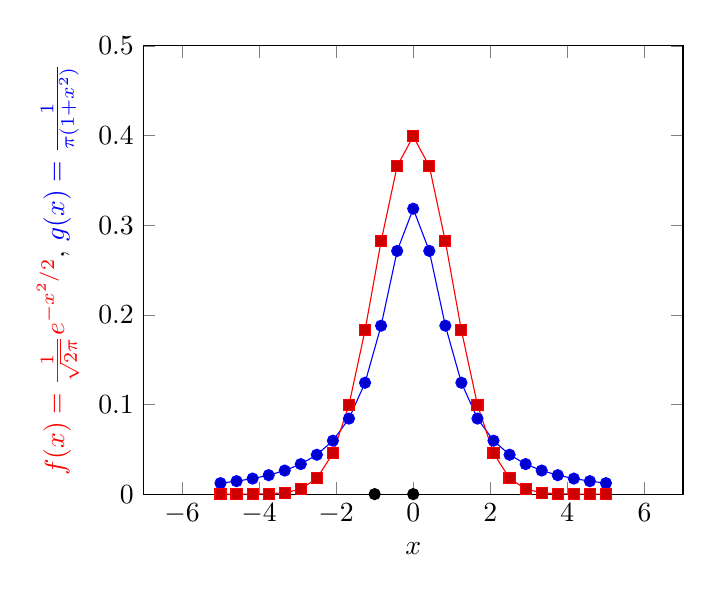
\begin{tikzpicture}
  \begin{axis}[ 
	xmin=-7,   xmax=7,
	ymin=0,   ymax=0.5,
    xlabel=$x$,
    ylabel={{\color{red}$f(x) =\frac1{\sqrt{2\pi}}e^{-x^2/2}$}, {\color{blue}$g(x)=\frac1{\pi(1+x^2)}$}}
  ] 
    \addplot {1/(pi*(1+x^2))}; 
    \addplot{e^(-x^2/2)/(2*pi)^(1/2)};
    \addplot [only marks,mark=*] coordinates { (-1,0) };
    \addplot [only marks,mark=*] coordinates { (0,0) };
    \addplot [only marks,mark=*] coordinates { (1,1) };
  \end{axis}
\end{tikzpicture}
\caption{The Cauchy distribution has ``heavier tails'' than the normal distribution.}
\end{figure}

\label{calculus}
\index{calculus|(}

\subsection{Limits}

$\lim_{x\to a}f(x)=L$ means that for each $\epsilon>0$, there is a $\delta>0$ such that for all $x$, if $0<|x-a|<\delta$ then $|f(x)-L|<\epsilon$.
The concept is used to define derivatives and integrals, but is also used directly in statistics, in the Law of Large Numbers and the Central Limit Theorem.

\subsection{Derivatives}

	The derivative $f'(x)=\frac{df}{dx}$ is defined by $\lim_{h\to 0}\frac{f(x+h)-f(x)}h$. The \term{Chain Rule} says that
	\[
		\frac{d}{dx}f(g(x))=f'(g(x))\cdot g'(x).
	\]
	The \term{Product Rule} says that
	\[
		\frac{d}{dx} f(x)g(x) = f'(x)g(x)+f(x)g'(x).
	\]
	Differentiation is a linear operation in the sense that
	\[
		\frac{d}{dx} cf(x)=cf'(x),\quad \frac{d}{dx}(f(x)+g(x)) = f'(x)+g'(x),
	\]
	where $c$ is a constant.

\subsection{Applications of derivatives}%: optimization}

	To find a maximum or minimum of $f(x)$, we solve the equation $f'(x)=0$ for $x$.
	If $f''(x)\ge 0$ (as is the case with the function $f(x)=x^2$) then we will have a minimum,
	and if $f''(x)\le 0$ (as with $f(x)=-x^2$) we will have a maximum.

	For a continuous random variable with pdf $f_X$, we can naturally define a \term{mode} to be
	any point $x$ with $f'_X(x)=0$ and $f''_X(x)\le 0$, i.e., a local maximum of $f_X$.

\subsection{Integrals}
	Integrals can be understood via the Fundamental Theorem of Calculus: $f(b)-f(a)=\int_a^b f'(x)\,dx$ and $\frac{d}{dx}\int_a^x f(t)\,dt=f(x)$.

	For discrete random variables with probability mass function $m(x)=\P(X=x)$, we require
	\[
	\sum_x m(x)=1,
	\]
	and analogously in the continuous case we need
	\[
	\int_{-\infty}^\infty f_X(x)\,dx=1
	\]
	when $f_X$ is the pdf of $X$.
\subsection{Applications of integrals}%: means}

	The mean of a random variable $X$ with pdf $f$ is $\int_{-\infty}^\infty x\,f(x)\,dx$.

	The expectation of $X^2$ is $\int x^2\,f(x)\,dx$, similarly.
	The general rule is that if $f_X$ is the pdf of $X$, and $g$ is any (deterministic, i.e., non-random) function, then
	\[
		\E(g(X)) = \int_{-\infty}^\infty g(x)\,f_X(x)\,dx.
	\]
\subsection{Inverse and trigonometric functions}%: $e^x$ and $\ln x$}

	The normal distribution (Exercise \ref{normal_dist}) and the exponential distribution use the exponential function $e^x$,
	which is related to the natural logarithm $\ln$ via
	\[
		y=e^x\iff \ln y=x
	\]
	where $y>0$.

	By the Chain Rule, if $y=f(f^{-1}(y))$ then
	\[
		1 = \frac{dy}{dy} = f'(f^{-1}(y))\cdot (f^{-1})'(y).
	\]
	This implies that, since $\frac{d}{dx} e^x=e^x$, using $f(x)=e^x$,
	\[
		\frac{d}{dy}\ln y = (f^{-1})'(y)=\frac1{f'(f^{-1}(y))} = \frac1{e^x} = \frac1y.
	\]
	Properties of logarithms generally follow from analogous ones for exponentials, e.g., the general rule
	\[
		\frac{\log_a x}{\log_a y} = \frac{\log_b x}{\log_b y}
	\]
	follows from the special case $b=y$:
	\[
		\frac{\log_a x}{\log_a y} = \frac{\log_y x}{\log_y y}
	\]
	(since this shows that the left hand side does not depend on $a$)
	which follows, using $a^{\log_a z}=z$, from
	\[
		\frac{\log_a x}{\log_a y} = \frac{\log_y x}{\log_y y}=\log_y x\iff \log_a y\log_y x = \log_a x
	\]
	\[
		\iff a^{\log_a y\log_y x} = a^{\log_a x}
		\iff (a^{\log_a y})^{\log_y x}=x
		\iff y^{\log_y x}=x.
	\]

\subsection{Techniques of integration}

Integration by parts $\int u'(x)v(x)\,dx=[u(x)v(x)]-\int v'(x)u(x)\,dx$ is often useful. % NOT for Exercise \ref{skewed} involving the skewed normal distribution.
Improper integrals $\int_{-\infty}^\infty f(x)\,dx$ are used for pdfs $f$.

\subsection{Applications of integration to probability}
The probability that $a\le X\le b$ is
\[
	\int_a^b f_X(x)\,dx
\]
where $f_X$ is the pdf~of $X$.

%\subsection{Differential equations}
%\subsection{Parametric equations and polar coordinates}

\subsection{Infinite sequences and series}
The geometric distribution is understandable after studying infinite series and in particular the geometric series
\[
	\sum_{n=0}^\infty x^n = \frac1{1-x},\quad |x|<1.
\]
When we check the 68-95-99.7 rule in Section \ref{997} we shall use Taylor series:
\[
f(x)=\sum_{n=0}^\infty \frac{f^{(n)}(0)}{n!}x^n.
\]